\section{提案手法}
既存手法の問題点として,ランダムな活性化関数の変更が挙げられる.探索後期において良いノードの出力の個体が生まれたとしても,例えば良いノードの活性化関数をlinear関数 $ f(x) = x $ からinverse関数 $ f(x) = -x $ に変更されてしまうと,ノードの出力は反転されてしまう.ネットワークの一部の構造化された部分の出力の大小は,同符号であれば出力層に大きな変化をもたらさないが,出力が0より大きいか小さいかは,ネットワークの出力は大きく変わることが知られている\cite{WANN}.\\
提案手法ではこれの問題を緩和するために,活性化関数の慎重な選択について言及する.2つの活性化関数の距離を計算し,距離が小さければ小さいほど変更先の活性化関数として選択されやすくなる.

\begin{figure}[h]
    \begin{center}
        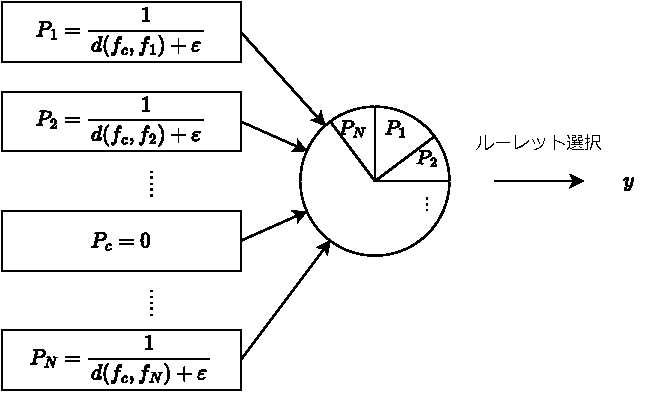
\includegraphics[scale=0.8]{img/exppropose.pdf}
        \caption{提案手法の概略図}
    \end{center}
\end{figure}

\begin{equation}
    P_{i} =  \begin{cases} \dfrac{1}{d(f_{c}, f_{i}) + \epsilon_{n} } \qquad (i \neq c) \\ 0 \qquad (i = c) \end{cases}\\
\end{equation}
\begin{equation}
    \epsilon_{n} = s * \epsilon_{n-1} \\
\end{equation}

\begin{table}[h]
    \caption{変数の説明}
    \centering
    \begin{tabular}{cl}
        \hline
        変数  & 意味 \\
        \hline \hline
        $P_{i}$               & $c$から$i$へ活性化関数IDが変更される見込み \\
        $d(f_{c}, f_{i})$     & 活性化関数が$c$と$i$の距離                 \\
        $f_{i}$               & IDが$i$の活性化関数                        \\
        $i$                   & 活性化関数ID                               \\
        $c$                   & 現在の活性化関数ID                         \\
        \hline
    \end{tabular}
\end{table}

まず現在の活性化関数 $ f_c $ と,すべての活性化関数との距離を計算する.この時の距離が小さいことは両者の関数が似ていることを意味し,距離の短い関数への変更は既存手法の問題点である出力の反転を防ぐ.距離が小さければ小さいほど選択されやすくするため,距離と $ \epsilon $ の和の逆数をルーレット選択の材料とする. $ \epsilon $ が大きくなると,ルーレット選択によって選ばれる確率はランダムに近くなる. $ \epsilon $ は探索初期においては,良いノードの出力を持つ個体が少ないことから,良い出力の個体を反転させてしまうデメリットより,悪い出力の個体を反転させるメリットの方が大きいと考え,探索初期の $ \epsilon $ は大きく,探索後期の $ \epsilon $ は小さく設定する.\\
距離関数 $ d $ については,区間積分差と,個体の経験に基づく出力差を採用する.

\subsection{活性化関数同士の区間積分差}
式(7)と式(8)は関数 $ f_a $ と $ f_b $ の範囲内の出力の差と,個体の経験に基づく出力差を意味している.

\begin{equation}
    d(f_{a}, f_{b}) = \int^{r}_{-r} (f_{a}(x) - f_{b}(x))^{2}
\end{equation}
\begin{equation}
    d(f_{a}, f_{b}) = \sum_{m}(f_{a}(in_{m}) - f_{b}(in_{m}))^2
\end{equation}

\begin{table}[h]
    \caption{変数の説明}
    \centering
    \begin{tabular}{cl}
        \hline
        変数  & 意味 \\
        \hline \hline
        $d(f_{a}, f_{b})$ & 活性化関数が$a$と$b$の距離                 \\
        $f_{i}$           & IDが$i$の活性化関数                        \\
        $m$               & ミニバッチサイズ x 共有重み                \\
        $in$              & 経験したノードに入力される値               \\
        $\epsilon_{n}$    & 探索範囲を考慮する                         \\
        $r$               & 関数の考慮範囲                             \\
        $k$               & $\epsilon$の減衰率,0.995など              \\
        \hline
    \end{tabular}
\end{table}

\subsection{個体の経験に基づく出力差}